\documentclass[a4paper]{article}
\usepackage{graphicx}
\usepackage[ngerman]{babel}
\usepackage[left=3.5cm, right=3cm, top=3cm, bottom=3cm]{geometry}
\usepackage{biblatex}
\usepackage{csquotes}

\bibdata{/Users/daniel/docs/LaTeX/misc/hadid-gfs/uni.bib}
\bibliography{/Users/daniel/docs/LaTeX/misc/hadid-gfs/uni.bib}


\begin{document}
\title{Zaha Hadid: Eine Architektin der Zukunft}
\author{Daniel Renschler}
\date{\today}
\maketitle

\begin{figure}[h]
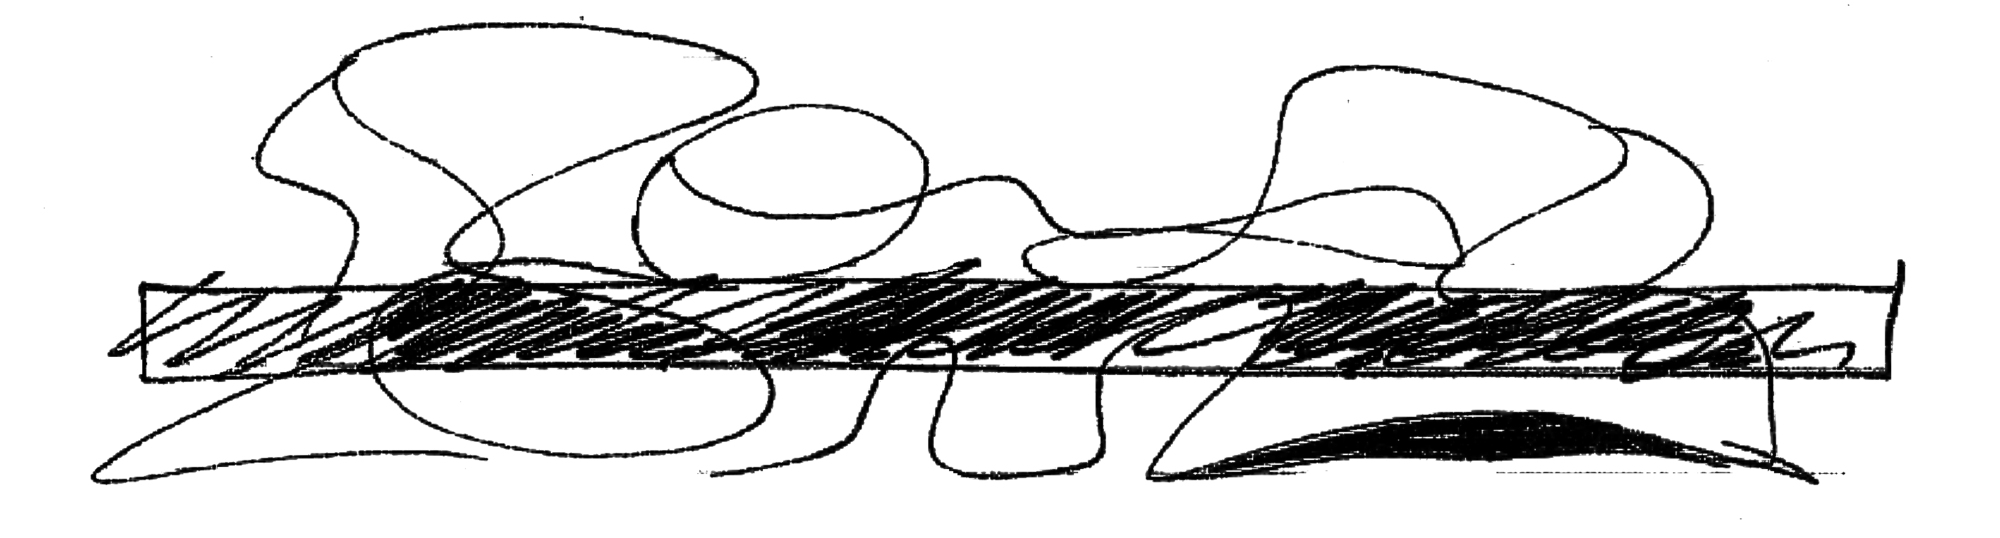
\includegraphics[width=\linewidth]{paeno-sketch.jpg}
\caption{Skizze Hadids für das pæno Wolfsburg\cite{article_creative_energy_sketches}}
\end{figure}

\begin{figure}[!h]
\centering
\large
Schuljahr 2022/–23, J1-1 \\
Fach: GMT \\
Lehrkraft: Frau Hildebrand \\
Rolf-Benz-Schule 

\end{figure}
\thispagestyle{empty}
\clearpage
\tableofcontents
\clearpage


\section{Einleitung}
\subsection{Kurzer Überblick über Zaha Hadids Leben und Karriere}
Zaha Hadid war eine irakisch-britische Architektin, die für ihre futuristischen
und kurvigen Designs bekannt war. Sie wurde 1950 in Bagdad geboren und studierte
Architektur in London an der Architekturschule der Architectural
Association.\cite{hadid_britannica}

Nachdem sie ihr Studium abgeschlossen hatte, gründete sie ihr eigenes
Architekturbüro in London und begann, ihre einzigartigen Designs zu entwickeln.
Sie wurde schnell für ihre innovativen und experimentellen Entwürfe bekannt und
gewann viele internationale Auszeichnungen.

Einige ihrer bekanntesten Projekte umfassen das London Aquatics Centre für die
Olympischen Spiele 2012, das Opernhaus Guangzhou und die Nord-Süd-Achse
der Biennale in Venedig. Sie war die erste Frau, die den Pritzker-Preis für
Architektur gewann, und wurde in vielen Auszeichnungen und Listen der
einflussreichsten Architekten der Welt aufgeführt~\cite{ZahaHadidAwards}.

Hadid starb 2016 im Alter von 65 Jahren, aber ihr Vermächtnis in der
Architekturwelt bleibt unbestreitbar. Sie wird als eine der bedeutendsten und
einflussreichsten Architekten des 21. Jahrhunderts betrachtet und ihre Arbeit
wird weiterhin in Museen und Ausstellungen auf der ganzen Welt gezeigt
\cite{hadid_britannica}.

\subsection{These (die den Hauptfokus der Arbeit zusammenfasst)}
Diese Arbeit versucht neben dem Leben und Projekten von Hadid grob
zusammenzufassen welchen Einfluss sie hatte mit ihrem parametrischen und
krummlinigen design auf Architektur des 21. Jahrhunderts.


\section{Frühes Leben und Ausbildung}
\subsection{Hadids Aufwachsen und Ausbildung}
Sie wuchs in einer wohlhabenden und künstlerisch orientierten Familie auf und
interessierte sich früh für Architektur und Kunst. Nach dem Abschluss der High
School studierte sie zunächst Mathematik an der American University in Beirut,
bevor sie Architektur an der Architekturschule des Architectural Association in
London studierte.

Während ihres Studiums entwickelte Hadid ihren unverwechselbaren Stil und ihr
Interesse an experimentellen Designs und fortschrittlicher Technologie. Sie
absolvierte ihr Studium mit Auszeichnung und begann anschließend ihre Karriere
als Architektin.

Hadids frühes Leben und ihre Ausbildung haben wesentlich dazu beigetragen, ihre
spätere Karriere und ihren unverwechselbaren Stil zu formen. Sie wurde von ihrer
künstlerisch orientierten Familie und ihrem Studium in Mathematik und
Architektur beeinflusst und hat diese Einflüsse in ihre spätere Arbeit
einfließen lassen.
\subsection{Frühe Einflüsse auf ihre Arbeit}
Zaha Hadid war von vielen verschiedenen Einflüssen während ihrer frühen Karriere
beeinflusst, die ihre Arbeit formten und prägten. Hier sind einige der
wichtigsten Einflüsse, die auf Hadids frühe Arbeit hatten:

\begin{itemize}
\item Mathematik: Hadid studierte Mathematik an der American University in Beirut,
bevor sie Architektur studierte. Sie war von der Schönheit und Präzision der
Mathematik fasziniert und setzte diese Einflüsse in ihre Architekturarbeit ein,
indem sie komplexe Formen und Kurven verwendete.
\item Kunst: Hadids Familie war künstlerisch orientiert und sie wurde von
verschiedenen Kunstrichtungen wie der abstrakten Expressionismus und der Kunst
der modernen Avantgarde beeinflusst. Diese Einflüsse waren in ihrer
Architekturarbeit deutlich zu sehen, insbesondere in ihrem unkonventionellen und
experimentellen Ansatz.
\item Architektur der Moderne: Hadid war von der Architektur der Moderne beeinflusst,
insbesondere von Architekten wie Le Corbusier und Ludwig Mies van der Rohe. Sie
schätzte die strenge Geometrie und das klare, funktionale Design dieser
Architekten und setzte diese Einflüsse in ihre eigene Arbeit um.
\item Fortschrittliche Technologie: Hadid interessierte sich für den Einsatz von
fortschrittlicher Technologie in der Architektur und verwendete häufig
innovative Materialien und Baumethoden in ihren Projekten. Dies trug dazu bei,
dass ihre Arbeit als futuristisch und avantgardistisch angesehen wurde.
\end{itemize}

\section{Bekannte Projekte und Designs}
\subsection{Überblick über einige der berühmtesten Projekte und Designs von Hadid}

\begin{itemize}
\item London Aquatics Centre: Das London Aquatics Centre war eines der
	Hauptspielstätten der Olympischen Spiele 2012 in London und beherbergt ein
	50-Meter-Schwimmbecken, ein 25-Meter-Schwimmbecken und ein
	Synchronschwimmbecken. Es ist für seine kurvigen Linien und sein
	futuristisches Aussehen bekannt.
\begin{figure}[h]
\centering
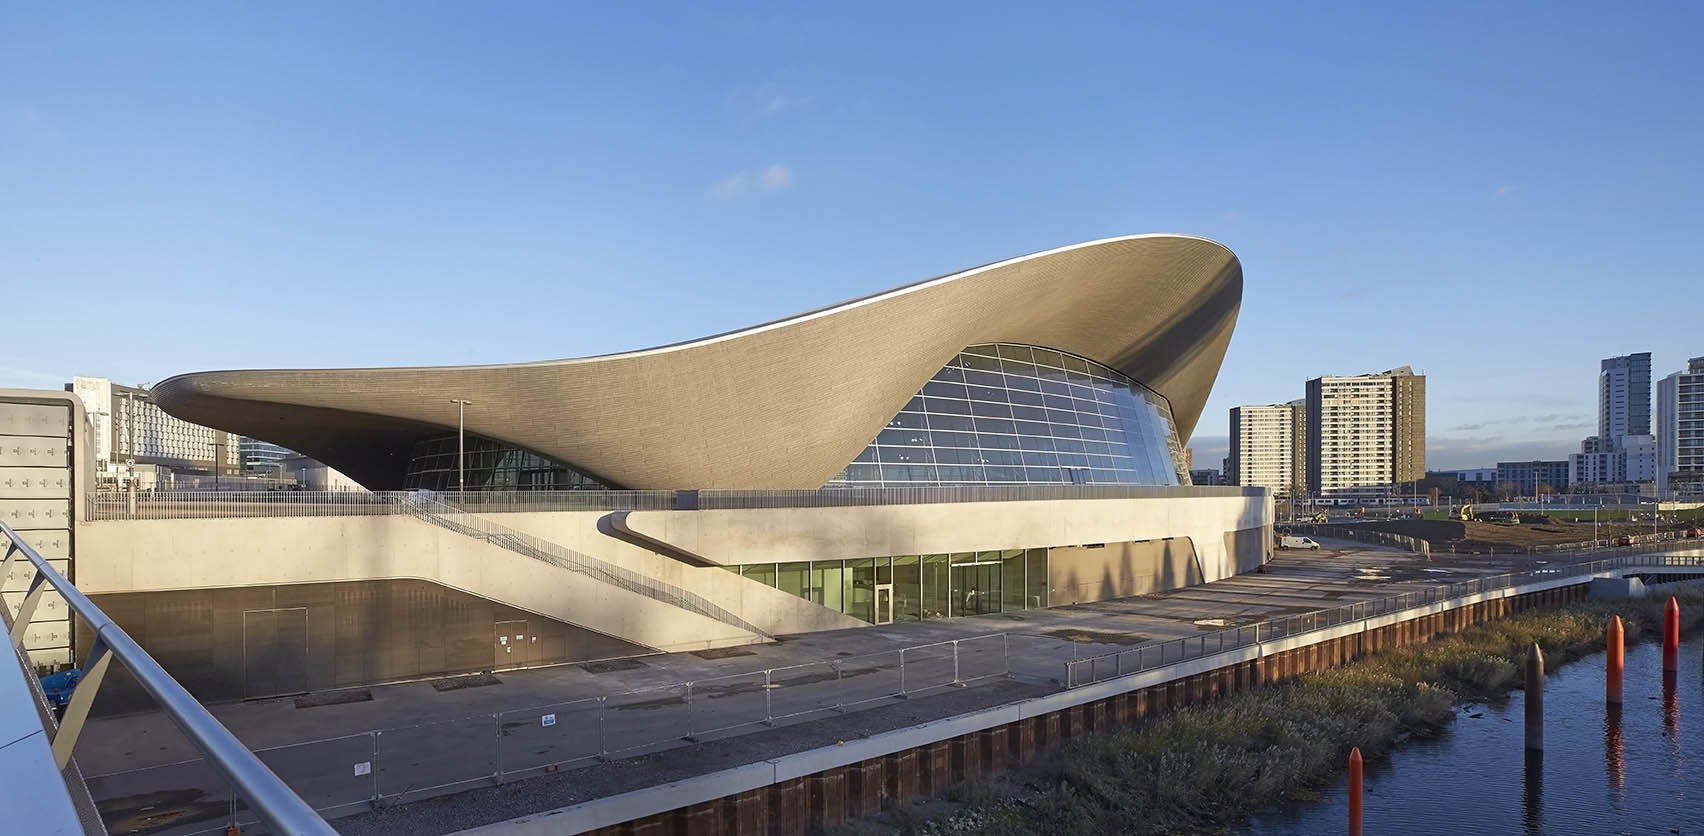
\includegraphics[width=.5\linewidth]{hadid-aquatics.jpg}
\caption{Das London Aquatics Centre von Hadid \cite{hadid_aquatics_centre}}
\end{figure}


\item Vitra-Feuerwache: Die Vitra Feuerwache in Weil am Rhein, Deutschland
	zeichnet sich durch ihre futuristische Architektur und langen geschwungenem
	Baukörper aus. Den Baukörper hat Hadid lang gezogen um das Vitra-Gelände von
	der benachbarten Bebauung abzuschirmen \cite[S. 26-29]{taschen_zaha_hadid}.
	Der Bau wurde aber nie als Feuerwache genutzt, stattdessen zeigt es die
	Offenheit für Architektur von Rolf Fehlbaum, der es in Auftrag gegeben hat.
\begin{figure}[h]
\centering
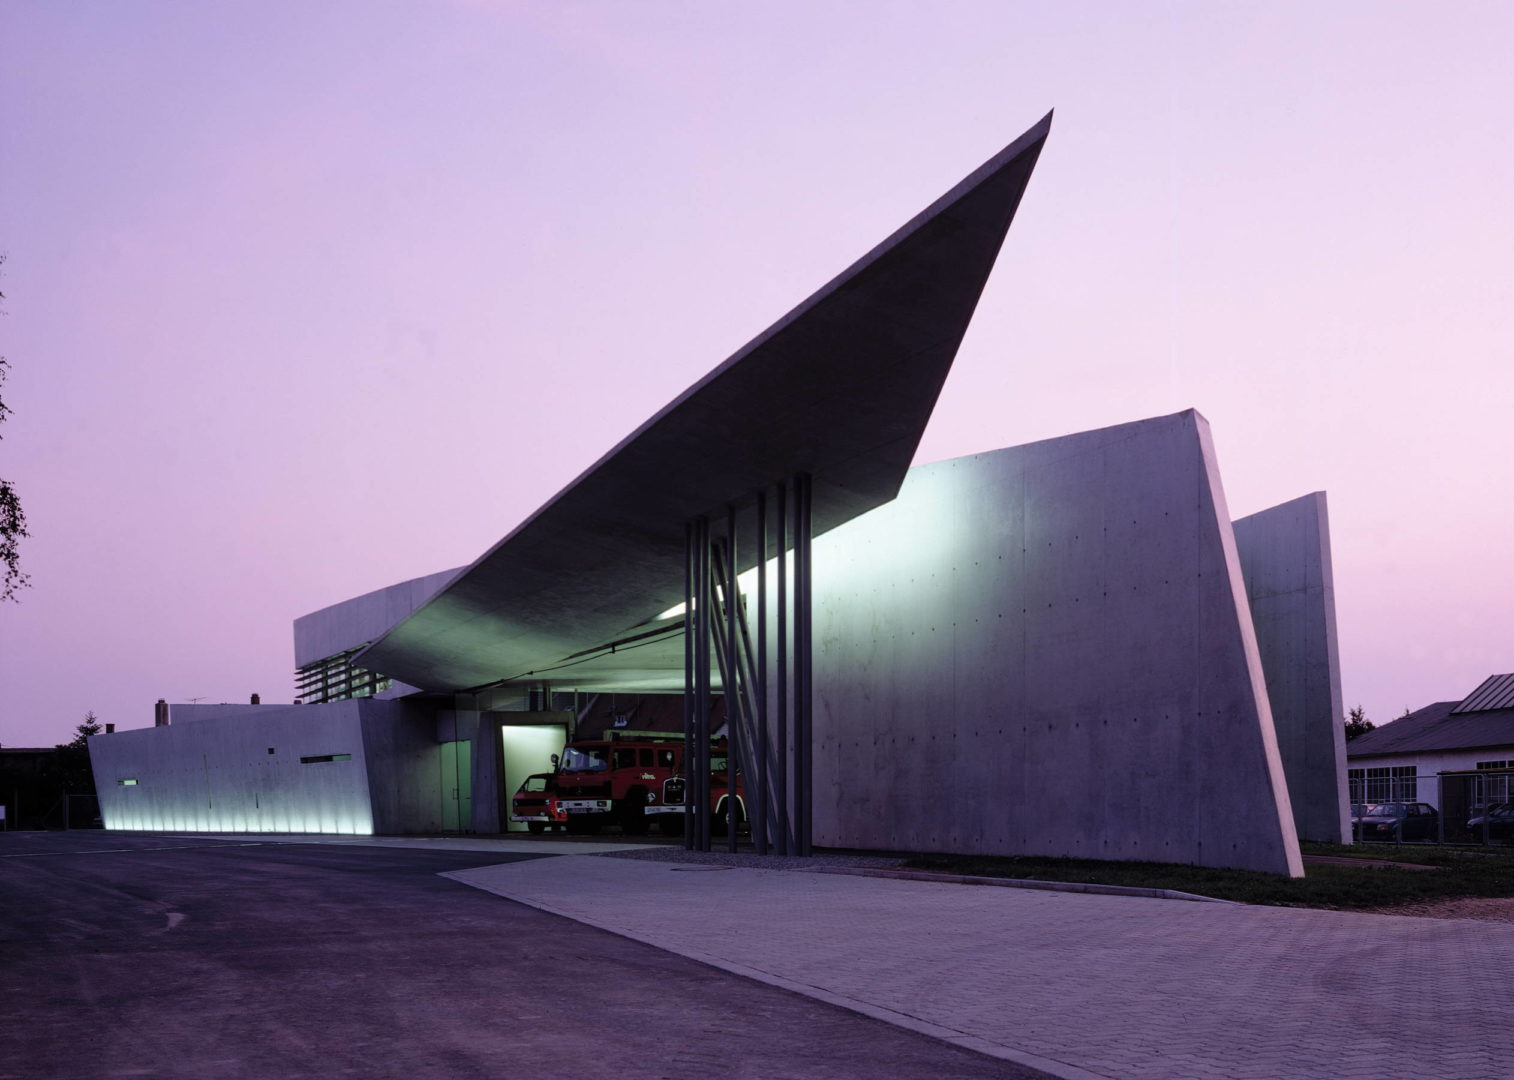
\includegraphics[width=.5\linewidth]{hadid-feuerwache.jpg}
\caption{Vitra Feuerwache \cite{hadid_vitra_fire_station}}
\end{figure}


\item Das Wolfburger Wissenschaftsmuseum phæno wurde von der Stadt Wolfburg und
	dem Gebäudenutzer Stiftung Phæno in Auftrag gegeben \cite[S.
	37]{taschen_zaha_hadid}. Besonderheiten sind die zehn Stützen die es halten,
	sodass es sich auf rund sieben Metern über dem Boden befindet. Außerdem
	reichen die Säulen durch das Gebäude und Stützen zusätzlich das Dach. Hadid
	sagt über das Bauwerk "Das Pæeno ist die bisher ehrgeizigste, umfassendste
	manifestation unserer Suche nach komplexen, dynamischen und fließenden Räumen.
	Der Besucher sieht sich einer Komplexität und Fremdheit gegenüber, die von
	einem sehr speziellen System gesteuert wird, das auf einer außergewöhnlichen
	volumetrischen strukturellen Logik gründet."
\begin{figure}[h]
\centering
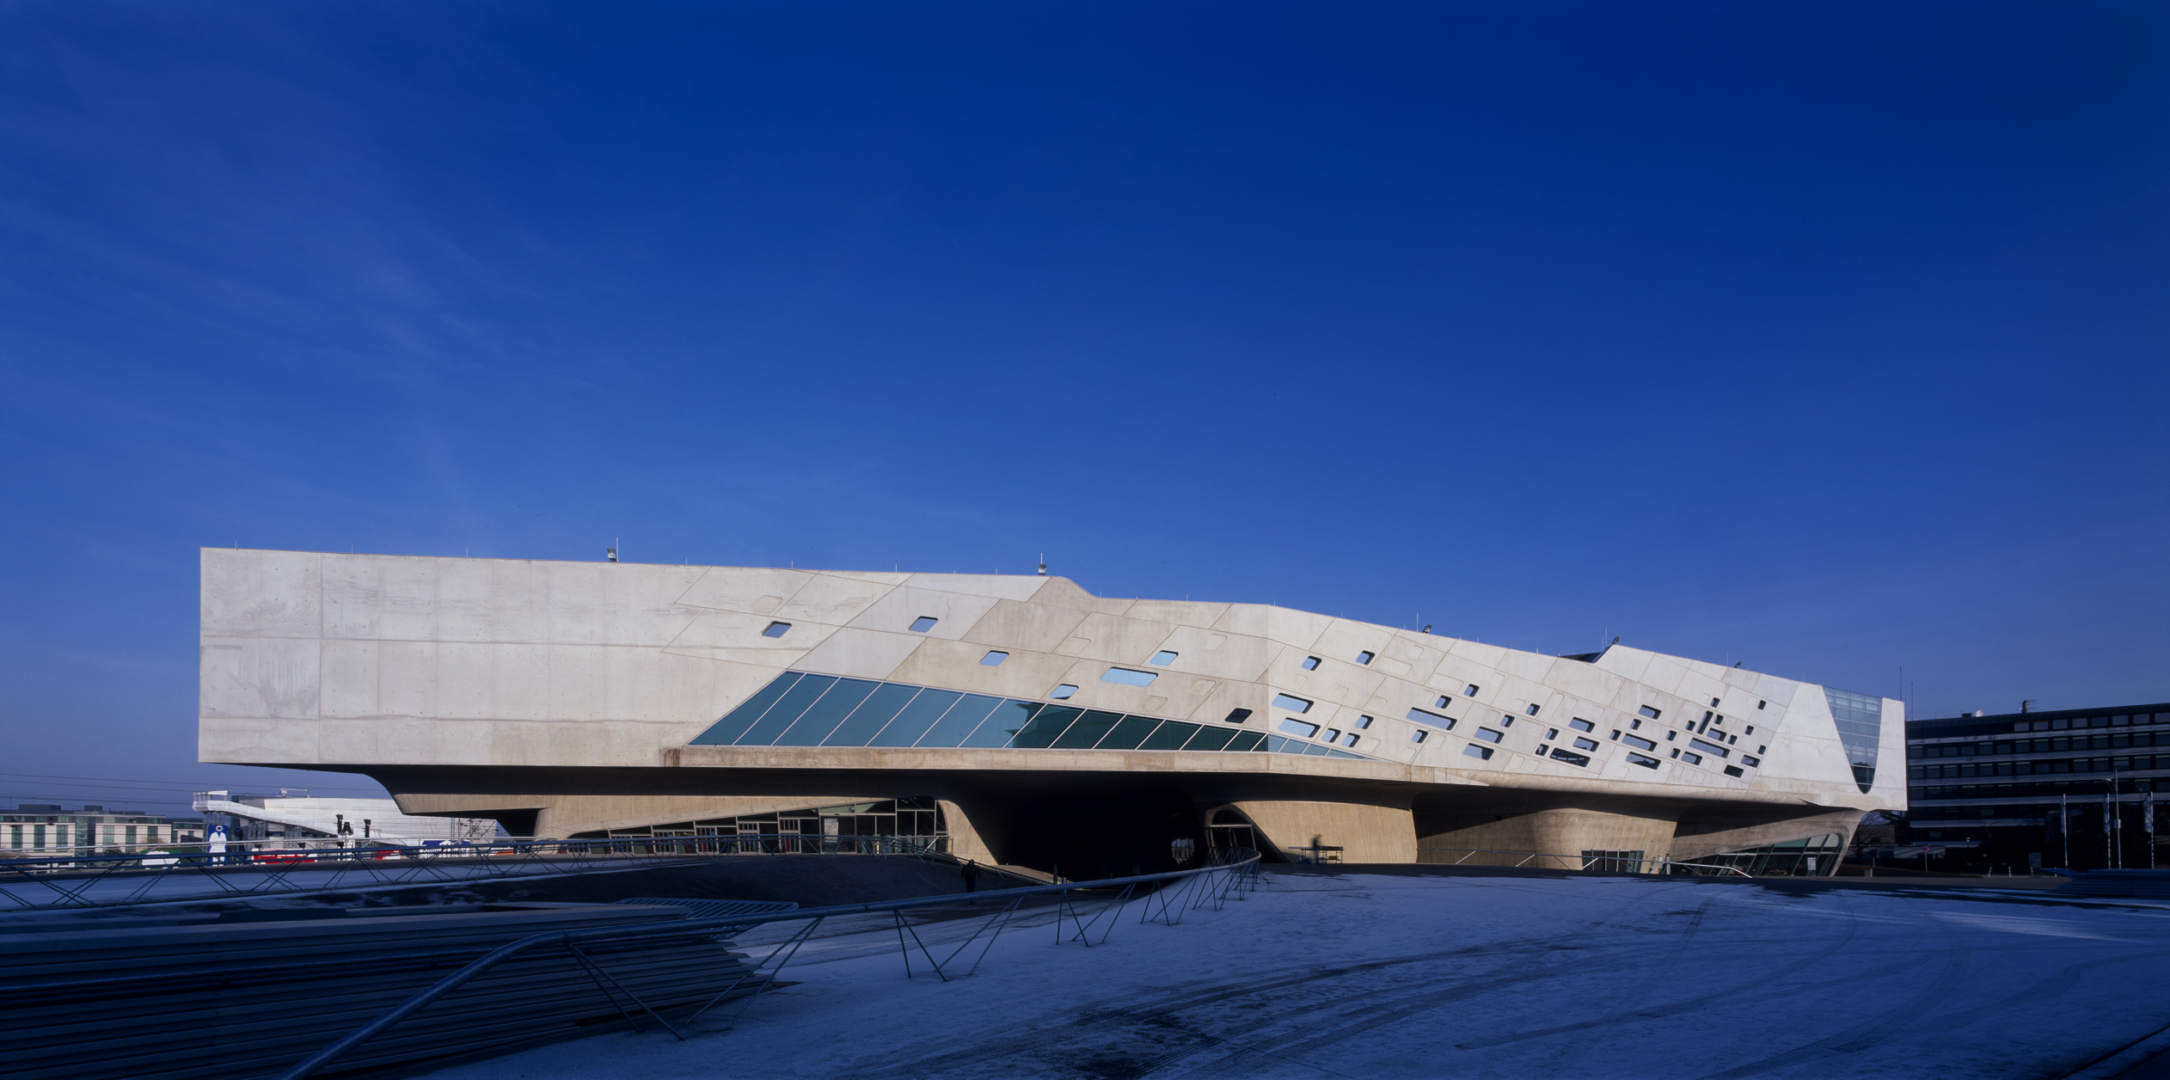
\includegraphics[width=.5\linewidth]{hadid-architects-phaeno.png}
\caption{Wissenschaftsmuseum phæno Wolfsburg \cite{hadid_phaeno_image}}
\end{figure}
\end{itemize}


\subsection{Analyse des Wissenschaftsmuseum phæno}
\begin{figure}[h]
\centering
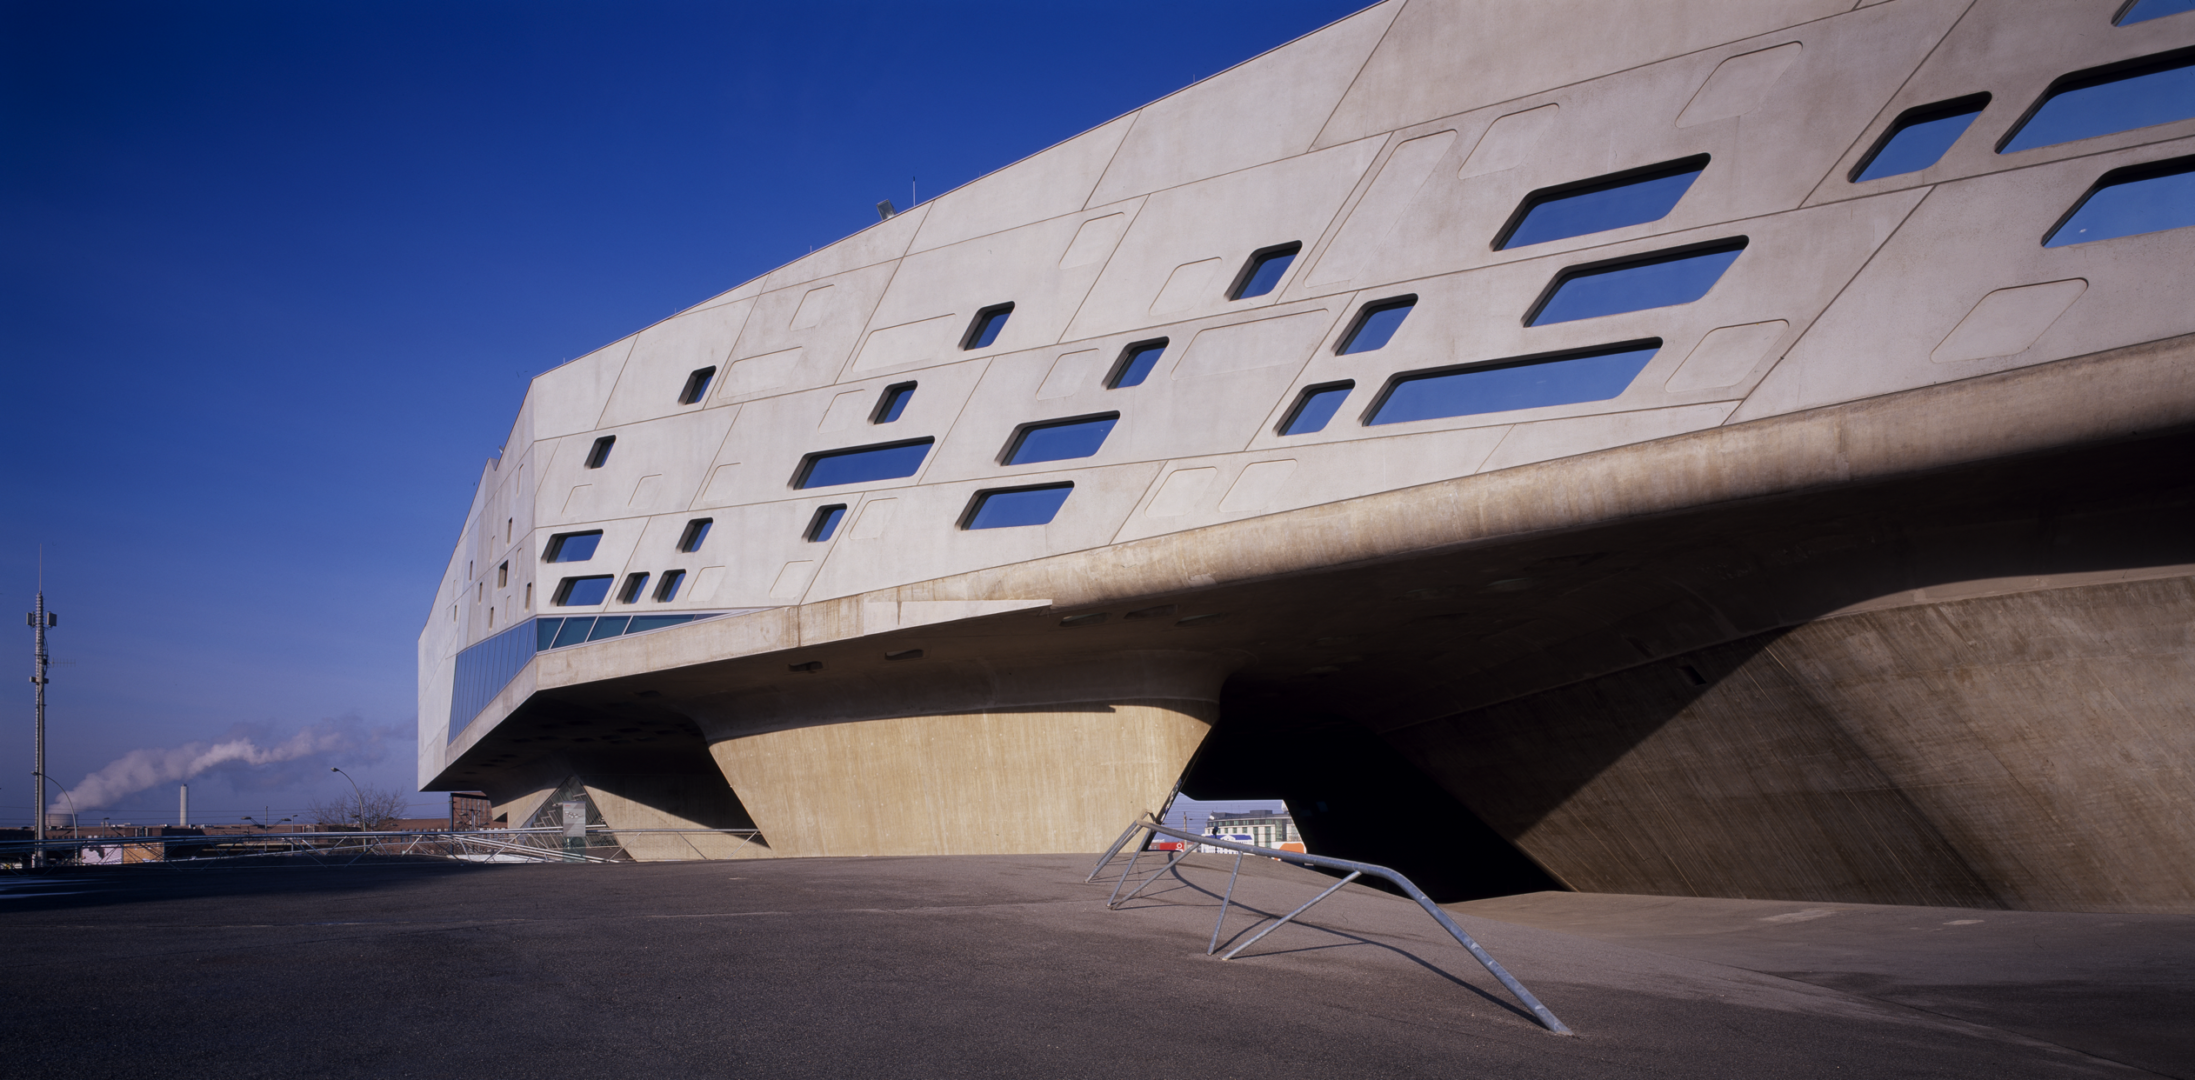
\includegraphics[width=\linewidth]{phaeno2.png}
\caption{Wissenschaftsmuseum phæno Wolfsburg \cite{phaeno2}}
\end{figure}
\subsubsection{Erster Eindruck}
groß, modern, hintergründig, seltsam
Beim ersten Blick war ich irritiert ob es nur ein riesiger Klotz auf Kegeln ist,
weil man das aus manchen Sichtwinkeln denken kann. Man versteht das Gebäude
nicht direkt, man braucht ein bisschen um zu verstehen wie es sich in der
Landschaft verhält und diese durch seine Kontinuität mit formt.

\subsubsection{Was ist dargestellt?}
Das Bauwerk "Wissenschaftsmuseum phæno" wurde entworfen von den Architekten
des Büros Zaha Hadid, London, und des Büros Mayer Bährle, Freiburg.
Es ist hauptsächlich aus Selbstverdichtendem Beton (SVB) \cite{Fulcrum} gegossen worden.
Außerdem ist es verstärkt mit einer unikem Stahl Kassettendecke. Das ganze ist
dann akzentiert durch Glas. Das Phœno bemaßt sich auf 154m x 130m x 97m mit
einer Höhe von 17m. Die begehbare Fläche beträgt sich auf ca. $11.000m^{2}$
\cite{KoppJenal2006}. Es gehört dem Architekturstil des parametrischem Design
an.

Das Phæno ist von der Grundfläche ein unregelmäßiges Viereck, welches eine
längste und kürzeste Seite hat welche verbunden sind, und restlichen Seiten sind durch zwei
mittellange Seiten geschlossen. Wenn man es aus bestimmten Winkeln sieht
erinnert das Museum auch an einen Schiffskörper der lang und hoch ist, ungefähr
150m lang und 17m hoch. Ein wichtiges Merkmal des Gebäudes ist, das es
auf zehn Konen steht, welche meist auch einen nutzen haben wie Eingang, Bistro,
Labor oder Restaurant. Dadurch ist der Hauptkörper des Phæno auf sechs bis zwölf 
Metern Höhe. Es ist gebaut, bzw. gegossen aus selbst verdichtendem Beton welcher bei diesem
Bauwerk das erste mal in Deutschland benutzt wurde. Betont ist es durch
Fenstern am Unterboden und an der Nord-West-Wand. Diese versorgen das Gebäude
aussorgend mit Licht und nicht wie üblich durch eine Überzahl an Leuchtmitteln,
die die Museumslandschaft visuell stören, trotzdem sind aber in der Stahl
Kassettendecke Lampen angebracht um die Ausstellungsstücke im Museums inneren zu
beleuchten bzw. auch die anderen wenn es dunkel ist.
\\––––––––––––––––––––––––––––––––––––––––\\
\subsubsection{Wie ist das Werk konzipiert}

\begin{figure}[h]
\centering
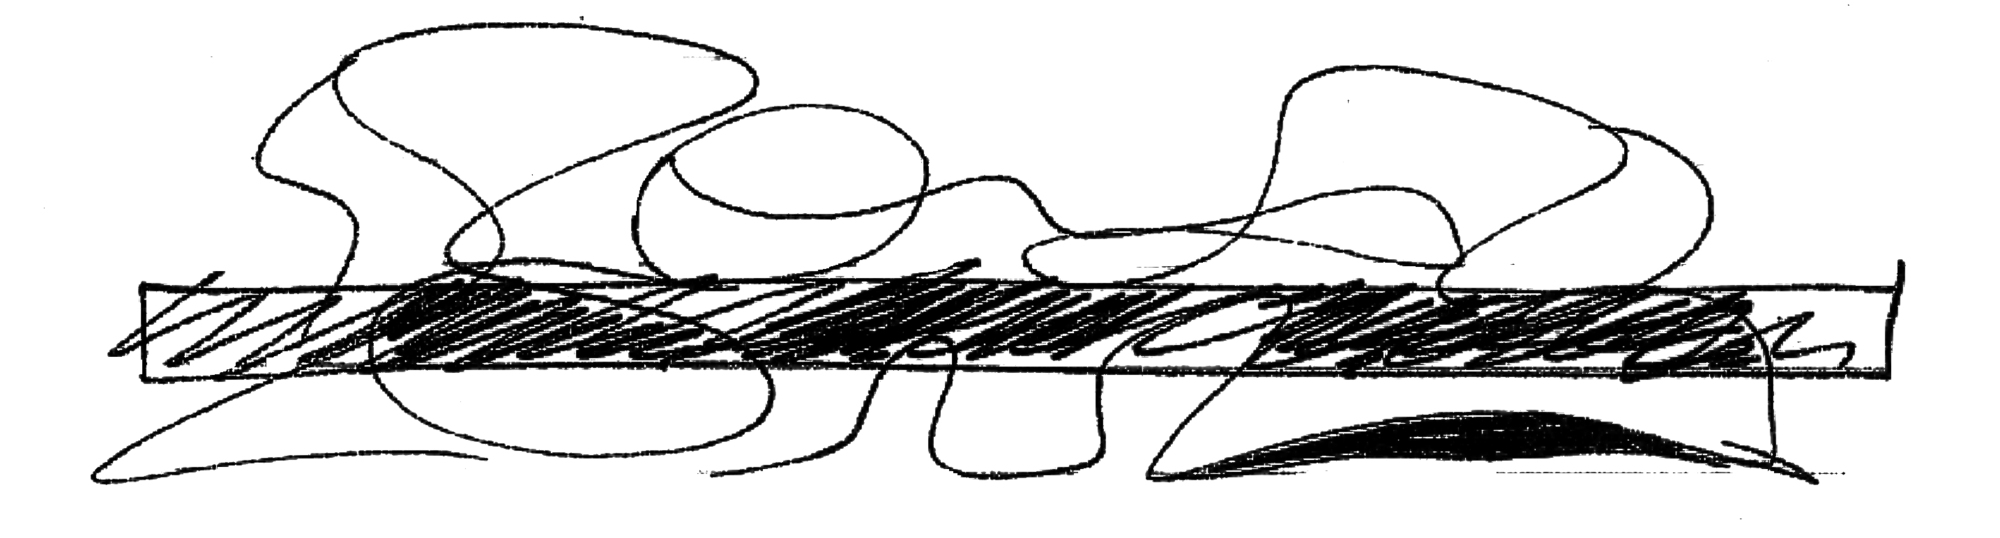
\includegraphics[width=.5\linewidth]{paeno-sketch.jpg}
\caption{Erste Skizze Hadids für das phæno.\cite{article_creative_energy_sketches}}
\end{figure}

Das werke wurde konzipiert in dem Rahmen eines Wettbewerb der Stadt Wolfsburg
welchen Hadid mit ihrem Büro dann 1999 gewann. Das phæno ist konzipiert wie auch
die meisten anderen Bauwerke Hadids, vergleichbar mit dem Guangzhou Opera House
durch 'computer-aided design' (CAD) und eine große Anzahl an Ilterationen um
auch das letzte detail genau zu beschreiben und illustrieren. Ihr Design 
allgemein ist geprägt von einem starken Schwerpunkt auf Innovation,
Experimentierfreude und dem Engagement, Werke zu schaffen, die die Grenzen
architektonischer Möglichkeiten ausloten wie beim phæno durch nutzen von
Selbstverdichtendem Beton und ein Gestell das ohne jedes einzelne Teil statisch
nicht möglich wäre. Dies braucht die größt mögliche Genauigkeit der Bauingeneure
und im vorfeld möglichst perfekte Vorarbeit der Architekten (hier Zaha Hadid
Arhcitects London \& dem Büro Mayer Bährle Freiburg).
Bei dem Bau wurden Schalungsformen für alle Teile des Gebäudes gebraucht um
den Selbstverdichtenden Beton zu nutzen, welcher vor der Härtung eine Konsistenz
vergleichbar mit Honig hat. Der wurde bei diesem Bauwerk wie schon früher
erwähnt das erste mal in Deutschland benutzt was es für das Lokale
Bauunternehmen sowie Ingeneure nicht einfacher machte. Das Glas welches benutzt
wurde war 3.3cm dick und in Länge und Höhe bis zu 4m x 6m, die Toleranz im
Beton lies aber nur 8mm Freiraum für diese für was die Schalen um so genauer
sein mussten und man sie keinen Fehler beim Bau und Herstellen der Scheibe
erlauben durfte. Der Beton ist Verantwortlich für starke Kanten an den Spitzen
und dem Hauptteil des Gebäudes, jedoch auch für weiche Konen die in das Gebäude
und Teilweise in den Boden übergehen und den Willy-Brand-Platz angenehm
begehbar machen.

Das Bauwerk wird nicht durch eine Zentrale Formensprache ausgezeichnet, es ist
kantig sowie abgerundet. Das einzige das es konstant einhält ist eine ferne von
rechten Winkeln oder Symmetrie was so gut wie alles von Zaha Hadid auszeichnet.

Das Bauwerk erfüllt seinen Zweck als Museum, Labor, Bistro und Restaurant. Es
füllt den Bauplatz auch wie geplant aus lässt aber trotzdem durch die Konen den
unterliegenden Willy-Brand-Platz frei, durch Glas im phæno und der 7-12 Metern erhöhten
Grundfläche ist hier auch noch genug Licht um den Platz für soziale Aktivitäten
zu nutzten, so wie auch jeden normalen Platz. Kriterien wie Ergonomie oder
Stapelbarkeit werden hier offensichtlich ausgelassen da es sich um ein Gebäude
handelt.
Form und Funktion sind nah einander, bei der Verleiung welcher Entwurf den
vorherig erwähnten Wettbewerb gewinnt sagte ein Juror ``Das Gebäude sieht auch wie
eine ``Mystery-Box', was Leute zur Besichtigung des Museums bringt, in dem sie
noch viel Naturwissenschaftliches erleben können werden außerhalb des
beeindruckenden Gebäudes.''
Das Material wurde gewählt um die unfassbaren Formen überhaupt verwirklichen zu
können und das diese für viele Jahre bestehen können.

Innovation sieht man nicht in diesem Gebäude, man kann es höchstens als
Innovation für deutsche Architektur sehen da man hier vorherig nicht
vergleichbares gesehen hat. Jedoch global gesehen ist es nur ein weiteres
Parametrisches Bauwerk in dem man dort keine besondere Innovation sieht.

\subsubsection{Resümee}
Resümierend kann man sagen das phæno Wolfburg ist zwar Deutschland weit eine
Innovation und ein Bautechnisches Meisterwerk, jedoch ist es global gesehen nur
ein weiteres Parametrisches Gebäude aus Zaha Hadids Vermächtnis. 

\section{Einfluss auf den Bereich der Architektur}

Sie war bekannt dafür, dass sie sich nicht an traditionellen Formen und
Konzepten in der Architektur gehalten hat und stattdessen ihren eigenen Weg
gegangen ist. Einige der wichtigsten Eigenschaften, die Hadid zu ihrem
Markenzeichen gemacht haben, sind:

\begin{itemize}
\item Fließende Formen und Linien: Hadid hat oft Gebäude entworfen, die sich
	durch ihre geschwungenen Linien und fließenden Formen auszeichnen. Sie hat die
	Grenzen dessen, was als möglich in der Architektur betrachtet wurde, immer
	wieder neu ausgelotet.
\item Bewegung und Dynamik: Hadids Gebäude haben oft den Eindruck von Bewegung
	und Dynamik vermittelt, auch wenn sie statisch sind. Sie hat dies erreicht,
	indem sie Linien und Formen verwendet hat, die sich in scheinbar unmöglichen
	Winkeln und Richtungen krümmen und verzerren.
\item Futuristisches Aussehen: Viele ihrer Gebäude haben ein futuristisches
	Aussehen gehabt, das durch die Verwendung von neuen Materialien und
	Technologien unterstützt wurde. Sie hat auch häufig Gebäude entworfen, die
	sich in ihre Umgebung einfügen, indem sie deren Landschaft, Klima und andere
	Eigenschaften berücksichtigt hat.
\item Innovation: Hadid war immer darauf bedacht, neue Wege zu gehen und die
	Grenzen der Architektur zu verschieben. Sie hat sich nicht an bestehenden
	Konzepten und Stilen orientiert, sondern hat stattdessen ihren eigenen Weg
	gegangen und viele innovative Ideen entwickelt.
\end{itemize}

Das ging soweit das Länder wie z.B. China ganze Designs von Hadid ``geklaut
habe'', bspw. mit einem Entwurf der ``MAD Architects'' für das National Museum
China welcher dann aber doch nicht gebaut wurde. 

Hadid war verantwortlich dafür das Software wie Rhino CAD (gut zum designen von
Parametrischem Design) und Maya (für Renderings) heute häufig benutzt werden
was für mehr vergleichbares Design sorgt, sozusagen war sie Vorreiter für ein
Design das grad noch am wachsen ist. Zaha Hadids Einfluss auf die Architektur
ist unbestreitbar, sie Prägte und entwickelte das parametrische CAD design von
Anfang an. Heute ist es presenter als je zuvor. Sie ein Gegner von jeder
Symmetrie und jedem rechten Winkel was
sie und ihre Arbeit ausmachte, sie benutzte auch am vermehrtesten andere
krummlinige Formen außerhalb von Bögen. Heute sind diese auch immer mehr
verbreitet in moderner Architektur. 

\section{Schlussfolgerung}
\subsection{Zusammenfassung der wichtigsten Punkte der Arbeit}
\begin{itemize}
	\item Brachte Krummlinige Formen außerhalb von Bögen in die Architektur.
	\item Machte CAD Software wir Rhino in den ``Mainstream'' was vergleichbare
		Architektur erst ermöglicht.
	\item Gab der Modernisierung der Architektur einen Rückenwind durch gewagte
		Designs.
	\item Designs sind so gut sie werden Regelmäßig geklont/geklaut.
\end{itemize}

\subsection{Abschließende Gedanken zum Einfluss und der Bedeutung von Hadid als
Architektin}
Hadid hatte einen großen Einfluss in die Moderne Architektur, es gibt immer mehr
Architekten die mit ihr als Vorbild nach dem Parametrischem Design Gebäude
entwerfen wie z.B. Philip Jodidio. Ihr Erbe bleibt bestehen mit ihrem
Architektur-Büro ``Zaha Hadid Architects, London'' welche auch nach ihrem Tod
weiter gemacht haben, und seitdem Bauwerke wie das ``National Museum XXI, Rom'',
den ``Bejing Daxing International Airport'' und vieles weiteres.


\clearpage
\section{Literatur}
\printbibliography



\end{document}
